\subsection{Introducción:}

En el siguiente ejercicio activaremos la páginacion básica. Completaremos el archivo \textit{mmu.c} para relizar los siguientes ítems.
\begin{itemize}
\item [\textit{a)}] Limpiar el buffer de video y pintar el mapa.
\item [\textit{b)}] Completar la función \textit{mmu\_mapear\_página(unsigned int virtual, unsigned int cr3, unsigned int física)}
\item [\textit{c)}] Utilizando la función anterior, completar la función \textit{mmu\_inicializar\_dir\_kernel} generar un directorio de páginas que mapee, usando identity mapping, las direcciones 0x00000000 a 0x003FFFFF. El directorio de páginas a inicializar se encuentra en la dirección 0x27000.
\item [\textit{d)}] Activar la paginación y verificar que el sistema sigue funcionando imprimiendo el nombre del grupo.
\item [\textit{e)}] Completar la función \textit{mmu\_unmapear\_pagina(unsigned int virtual, unsigned int cr3)}
\item [\textit{f)}] Probar la función anterior desmapeando la última página del kernel (0x3FF000).
\end{itemize}

\subsection{Ítem a): Limpiar el buffer de video y pintar el mapa \textit{IDT}}

Este ítem ya lo implementamos anteriormente, el mapa ya se encuentra pintado. Lo hicimos en el ejercicio 2, al utilizar las funciones  \textit{aux\_limpiarPantalla} y \textit{screen\_inicializar}. \\

\subsection{Ítem b): Completar la función \textit{mmu\_mapear\_página(unsigned int virtual, unsigned int cr3, unsigned int física)}}

En este punto realizamos la siguiente función: 

\begin{figure}[H]
\begin{center}
\minipage{1.0\textwidth}
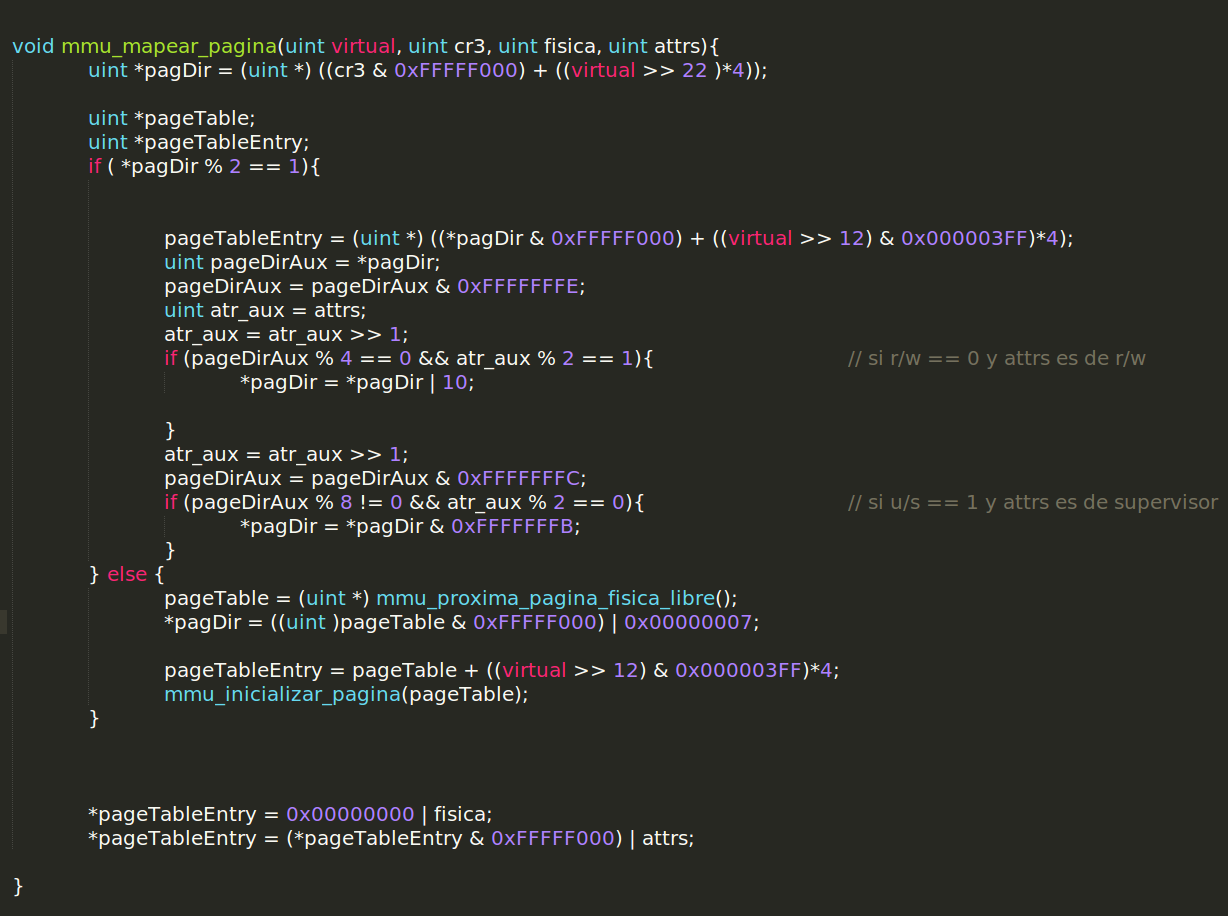
\includegraphics[width=\linewidth]{ejercicio3/mappag.png}
\caption{{\small Función mapeadora} }
\endminipage
\end{center}
\end{figure}

Lo que realiza esta función es lo siguiente: 

\begin{itemize}
	\item[A:] Recibe como parámetro una dirección virtual, una física, un \textit{CR3} y la informacion sobre los atributos. 

	\item[B:] Como \textit{CR3} tiene la siguiente forma:
	 
	 \begin{figure}[H]
	 \begin{center}
	 \minipage{0.6\textwidth}
  	 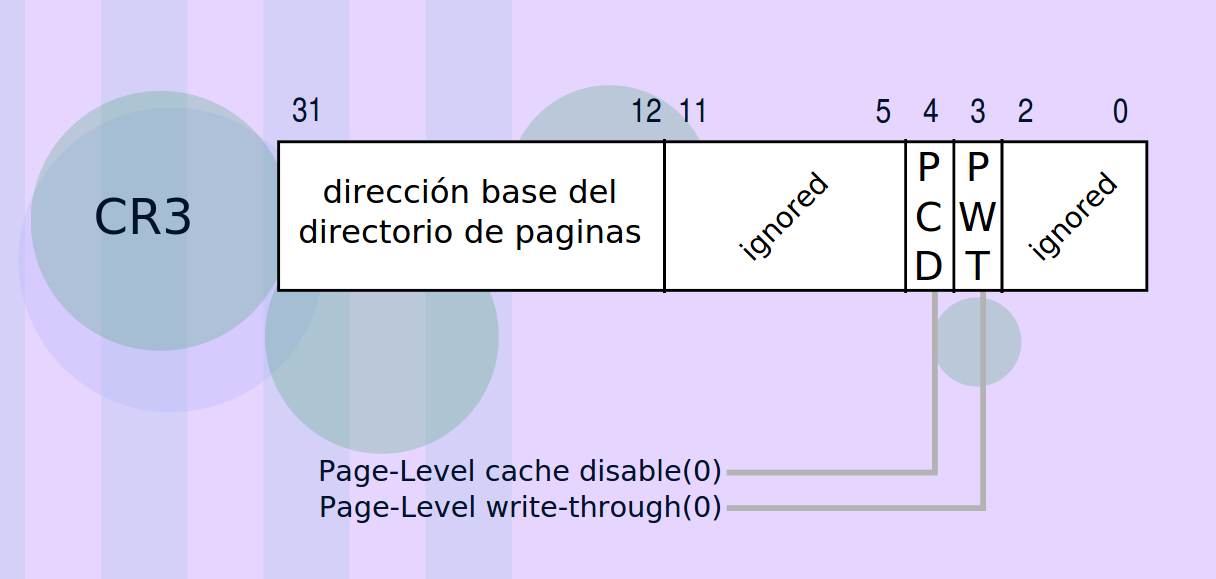
\includegraphics[width=\linewidth]{ejercicio3/cr3.png}
  	 \caption{{\small Formato \textit{CR3} }}
	 \endminipage
	 \end{center}
	 \end{figure}

	  Le hacemos un and lógico con 0xFFFFF000, de esta forma nos quedamos solo con la direccion base del directorio de páginas del cr3. Luego shifteamos la direccion virtual del parámetro de entrada en 22 posiciones, para quedarnos con el offset de la misma y multiplicamos este offset por 4 pues los punteros de las páginas de directorio ocupan 32 bytes y cada posicion de memoria es de 8.\\

	  Ahora sumamos la direccion base del directorio de páginas con el offset anterior y obtenemos la dirección de la tabla de página que buscabamos.

	 \begin{figure}[H]
	 \begin{center}
	 \minipage{0.8\textwidth}
  	 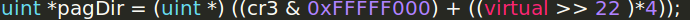
\includegraphics[width=\linewidth]{ejercicio3/fun1.png}
  	 \caption{{\small Formato \textit{CR3} }}
	 \endminipage
	 \end{center}
	 \end{figure}

	 \item[C:] Lo siguiente es fijarse si la direcion de la tabla de página obtenida existe o no. Para esto nos fijamos que en modulo 2 la direccion anterioirmente obtenida. Asi obtenemos el útlimo bit de la misma, si es 1 (P) sabemos que esta presente y si es 0 sabemos que no lo esta ($\neg$P) y tenemos que crearla
	 \begin{itemize}
	  \item[P: ] Si esta presente, tenemos que encontrar la posición de la tabla de página deseada. Para eso, realizamos un and lógico con la dirección obtenida anteriormente y  0xFFFFF000 para obtener la direccion base de la tabla de página (en la cual buscaremos la posicion deseada).

	 \begin{figure}[H]
	 \begin{center}
	 \minipage{0.6\textwidth}
  	 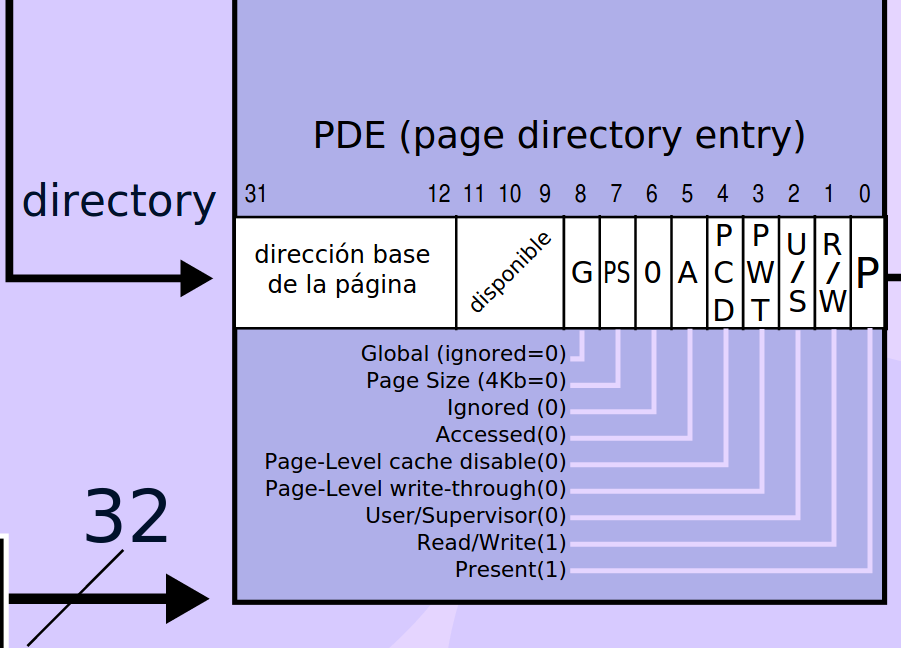
\includegraphics[width=\linewidth]{ejercicio3/fun2.png}
  	 \caption{{\small Formato de una posicion del directorio de tabla de páginas}}
	 \endminipage
	 \end{center}
	 \end{figure}

	  Luego shiftemos 12 posiciones la direccion vitual del parámetro de entrada para obtener el segundo offset necesesario y le hacemos un and lógico con 0x000003FF ara que solo quede la informacion que queremos y limpiar la posible basura que haya. \\

	  Este offset lo multiplicamos por 4 por la misma razón explicada anteriormente y se lo sumamos a la direccion base obtenida antes. Asi obtenemos la posicion de la tabla de página deseada.\\

	  En este caso, es necesario checkear si los atributos que se encuentran en la posicion recientemente encontrada son los mismos que los que se encontraban en la posicion del directorio de páginas encontrada en B. Obtenemos los atributos, y los comparamos, y en caso de ser necesario los cambiamos. \\

	  \begin{figure}[H]
	  \begin{center}
	  \minipage{0.6\textwidth}
  	  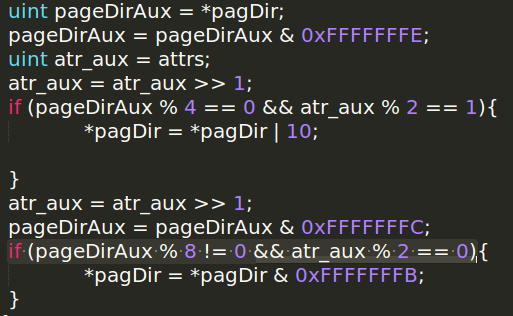
\includegraphics[width=\linewidth]{ejercicio3/fun3.png}
  	  \caption{{\small Comparacion y cambio de atributos}}
	  \endminipage
	  \end{center}
	  \end{figure}


	  \item[$\neg$P: ] Si la página no estaba presente, en necesario crearla. Entonces pedimos una dirección para crearla con la función \textit{mmu\_proxima\_página\_fisica\_libre()}. Luego ponemos esta direccion obtenida en el directorio de tabla de páginas, en la posicion obtenida en B, con los atributos correspondientes (para eso el or lógico con 0x00000007 )\\

	  \begin{figure}[H]
	  \begin{center}
	  \minipage{0.5\textwidth}
  	  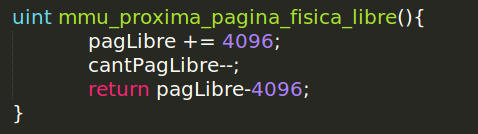
\includegraphics[width=\linewidth]{ejercicio3/proxpaglibre.png}
  	  \caption{{\small Función que nos da una posicion libre para poner una página. La variable pagLibre es una variable global inicializada con el valor 0x100000, y cantPaglibre en 768}}
	  \endminipage
	  \end{center}
	  \end{figure}

	  Por último obtenemos la posicion deseada de la tabla de página obtenida en B de la misma manera que cuando la página esta presente e incicializamos la tabla de página llenandola de ceros.

	   \begin{figure}[H]
	  \begin{center}
	  \minipage{0.5\textwidth}
  	  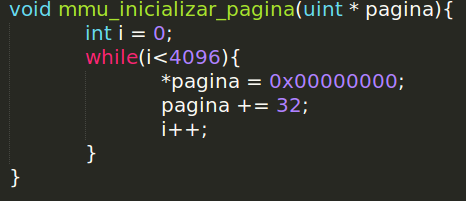
\includegraphics[width=\linewidth]{ejercicio3/inicializarpag.png}
  	  \caption{{\small Función que inicializa una página}}
	  \endminipage
	  \end{center}
	  \end{figure}

	 \end{itemize}

	 \item[D:] Ahora que tenemos todo en orden y la posición de la tabla de página deseada, procedemos a poner en esta posición la direccion física pasada por parámetro con los atributos tambien pasados por parámetro.

	  \begin{figure}[H]
	  \begin{center}
	  \minipage{0.6\textwidth}
  	  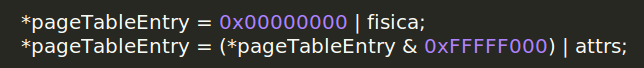
\includegraphics[width=\linewidth]{ejercicio3/fun4.png}
  	  \caption{{\small Identity mapping}}
	  \endminipage
	  \end{center}
	  \end{figure}

	  Como es Identity Mapping alcanza con poner en esta posición el resultado de hacer un or lógico con la direccion física y luego un or lógico con los atributos.

\end{itemize}
	  
	  \subsection{Ítem c): Inicializar el directorio de páginas en 0x00027000  y mapear las direcciones desde la 0 hasta la 0x003FFFFF con Identity Mapping\textit{IDT}}

	  Para realizar lo pedido completamos la funcion \textit{mmu\_inicializar\_dir\_kernel} mostrada a continuación:

	  \begin{figure}[H]
	  \begin{center}
	  \minipage{0.7\textwidth}
  	  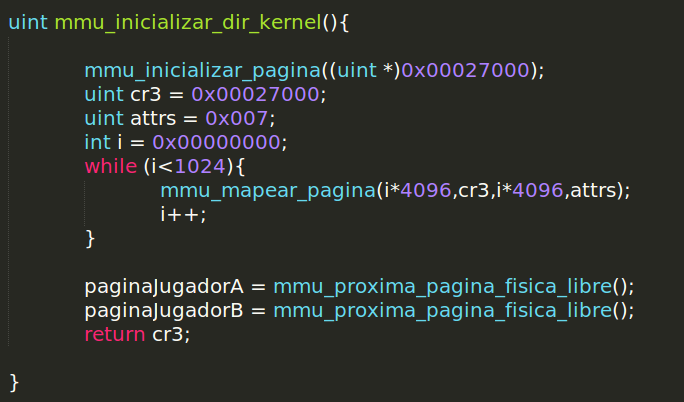
\includegraphics[width=\linewidth]{ejercicio3/inikernel.png}
  	  \caption{{\small }}
	  \endminipage
	  \end{center}
	  \end{figure}

	  Esta funcion comienza creando una tabla de páginas vacía en la dirección 0x27000, la cual va a actuar como directorio de páginas. Luego crea la variable \textit{Attrs} y la inicializa con el valor 0x007, el cual corresponde a los atributos que queremos que tenga el directorio de páginas, osea que P = 1, sea de lectura y escritura y sea de sistema. Tambien crea la variable \textit{Cr3} el cual se le asigna el valor  0x00027000 para que tenga la direccion base y los atributos correspondientes al directorio de paginas que queremos inicializar.\\

	 Para mapear cada posición del directorio recientemente creado se llama a la función del ítem anterior . LLamamos a esta función con las variables  \textit{Cr3} y \textit{Attrs} anteriormente creadas, y en cada iteracion se le da una posicion nueva del directorio para que haga el correpsondiente mapeo. \\

	 Por último es necesario que cada jugador tenga una página, por eso le asignamos a cada uno una página libre.

\subsection{Ítem d): Activar la paginación y verificar que el sistema sigue funcionando imprimiendo el nombre del grupo.}

	Activamos la paginacion escribiendo en el kernel las siguientes líneas:

	\begin{center}
    	$~$  \\ 	 
	Inicializar el directorio de paginas: \\
	$~$  \\ 	 
  	call mmu\_inicializar\_dir\_kernel  $~~~~~$  \\ 

  	$~$  \\ 
    	Cargar directorio de paginas:  $~~~~~~$  \\
    	$~$  \\ 

    	mov eax, 0x00027000  $~~~~~~~~~~~~~~~~~$  \\
    	mov cr3, eax  $~~~~~~~~~~~~~~~~~~~~~~~~~~~~$  \\

    	$~$  \\ 
    	Habilitar paginacion:  $~~~~~~~~~~~~~~~~$  \\
       	$~$  \\ 
   
        	mov eax, cr0  $~~~~~~~~~~~~~~~~~~~~~~~~~~~~$  \\
    	or eax, 0x80000000  $~~~~~~~~~~~~~~~~~~~$  \\
    	mov cr0, eax  $~~~~~~~~~~~~~~~~~~~~~~~~~~~~$  \\

	\end{center}

	Luego verificamos que el sistema sigue funcionando imprimiendo por pantalla el nombre del grupo

	  \begin{figure}[H]
	  \begin{center}
	  \minipage{0.9\textwidth}
  	  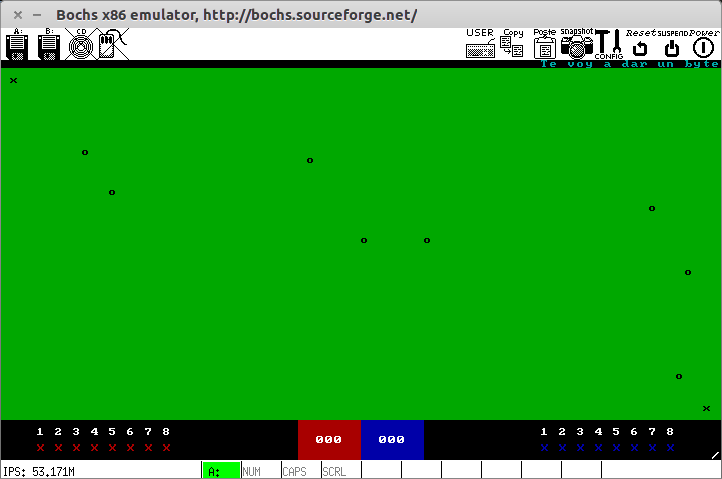
\includegraphics[width=\linewidth]{ejercicio3/nombre.png}
  	  \caption{{\small }}
	  \endminipage
	  \end{center}
	  \end{figure}

\subsection{Ítem e): Completar la función \textit{mmu\_unmapear\_pagina(unsigned int virtual, unsigned int cr3)}}

	Para unmapear una dirección virtual realizamos la siguiente función 

	  \begin{figure}[H]
	  \begin{center}
	  \minipage{0.9\textwidth}
  	  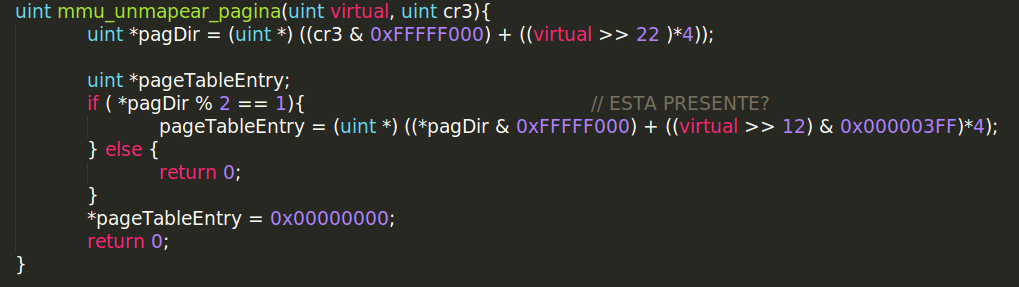
\includegraphics[width=\linewidth]{ejercicio3/unmap.png}
  	  \caption{{\small Identity mapping}}
	  \endminipage
	  \end{center}
	  \end{figure}

	La cual realiza el mismo cálculo que en el ítem 2 para acceder a la posicion de tabla de pagina buscada en el directorio de páginas y luego si esta pagina esta presente se hace un calculo tambien explicado anteriormente para acceder a la posicion deseada en esta pagina. Una vez obtenida esta posicion se procede a llenarla con ceros.


\subsection{Ítem f): Probar la función anterior desmapeando la última página del kernel (0x3FF000).} 

	 Para probar la función anterior, escribimos en el kernel las siguientes lineas:
	 \begin{center}

	 $~$  \\ 
	 Le pasamos los parametros a la funcion: \\
	 $~$  \\ 
	 mov eax, cr3 $~~~~~~~~$\\
   	 push eax$~~~~~~~~~~~~~~$ \\
   	 mov eax, 0x3FF000 \\
   	 push eax $~~~~~~~~~~~~~$\\

   	 $~$  \\ 
   	 La llamamos:\\
   	 $~$  \\ 
   	 call mmu\_unmapear\_pagina \\

   	 $~$  \\ 
   	 Limpiamos pila:\\
             $~$  \\ 
  	 pop eax \\
  	 pop eax \\
	 \end{center}

	 De esta manera llamamos a la función, y para ver que los resultados son los deseados, usamos el comando \textit{Info tab} de \textit{bochs} para ver hasta donde llega el mapeo de paginas y obetemos que llega hasta la direccion 0x3FEFFF en vez de llegar hasta 0x3FEFFF, por lo tanto podemos decir que la función hizo lo devido.
 
	  \begin{figure}[H]
	  \begin{center}
	  \minipage{0.9\textwidth}
  	  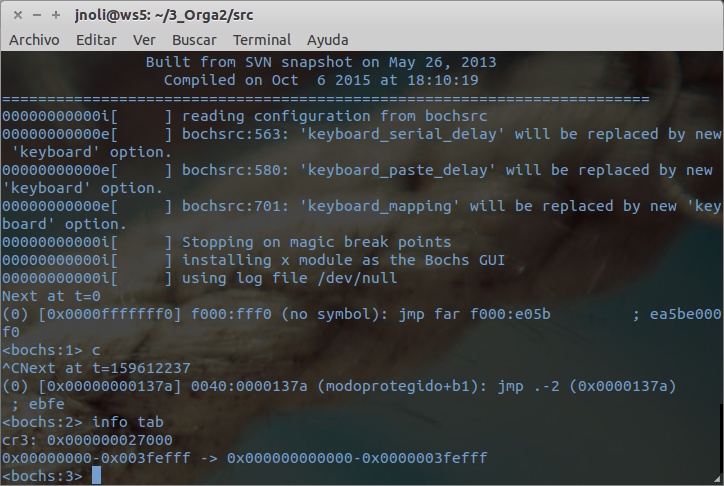
\includegraphics[width=\linewidth]{ejercicio3/unmaproof.png}
  	  \caption{{\small Identity mapping}}
	  \endminipage
	  \end{center}
	  \end{figure}
	




